\documentclass[10pt]{beamer}

\usetheme{m}

\usepackage{booktabs}
\usepackage{graphicx}
\usepackage[scale=2]{ccicons}

\usepackage{pgfplots}
\usepgfplotslibrary{dateplot}

\title{Git Submodules}
\subtitle{An intro to managing dependencies}
\date{\today}
\author{Miguel Gonzalez and Jan Kerkenhoff}
\institute{Fontys Hogeschool Venlo}
% \titlegraphic{\hfill\includegraphics[height=1.5cm]{logo/logo}}

\begin{document}

\maketitle

\begin{frame}
  \frametitle{Table of Contents}
  \setbeamertemplate{section in toc}[sections numbered]
  \tableofcontents[hideallsubsections]
\end{frame}


\section{Introduction}

\begin{frame}
  \frametitle{Monoliths (really big projects!)}
  \begin{center}
\includegraphics[width=280px]{images/monoliths.jpg}\end{center}
\end{frame}

\begin{frame}
  \frametitle{Monoliths (continued)}
  In terms of \textbf{git} there are a lot of drawbacks:
  \begin{itemize}
  	\item takes a long time to clone
  	\item many contributors
  	\item hard to keep track of all changes
  	\item wastes local disk space
  \end{itemize}  
\end{frame}

\begin{frame}
  \frametitle{the answer to everything: git-submodules!}
  \begin{center}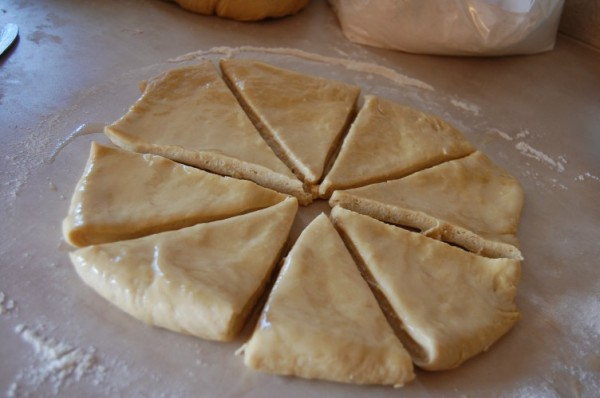
\includegraphics[width=200px]{images/divide.jpg}\end{center}
  \begin{center}\textbf{git submodule }add $<$repository-url$>$\end{center}
\end{frame}

\begin{frame}
	\frametitle{Sounds awesome, doesn't it?}
	Submodules let devide your repository into smaller parts.
	\begin{itemize}
		\item each submodule can be cloned individually.
		\item pushed commits from a submodule go directly to the specified origin (of the submodule).
		\item easy to distinguish between different projects (divided into multiple repositories)
		\item no disk space waste, only file with pointers exist.
	\end{itemize}
\end{frame}

\section{Updating Submodules}
\section{Working on Submodules}

\begin{frame}
	\frametitle{digging deeper..}
	\begin{itemize}
		\item When initializing a submodule, a \textbf{.gitmodules} file will be created. It contains a \emph{SHA1} commit id.
		\item \textbf{git-grep} does not look for submodules.
		\item update via \textbf{git submodule update}
		\item committing in a submodule does not update the \textbf{.gitmodules} file!
	\end{itemize}
\end{frame}

\section{Live Demo}

\begin{frame}
	\frametitle{Sounds awesome, doesn't it?}
\begin{center}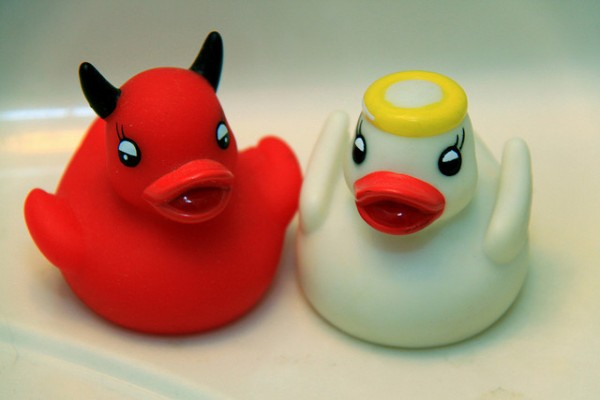
\includegraphics[width=280px]{images/goodbad.jpg}\end{center}
\end{frame}

\section{Pros and Cons}

\begin{frame}
  \frametitle{Pros (the strength)}
  
\end{frame}

\begin{frame}
	\frametitle{Cons (well..)}
\end{frame}

\section{Alternative: subtrees}

\end{document}